\chapter{Planteamiento del problema} 

La diversidad cultural es la multiplicidad de formas en que se expresan las culturas de los grupos y de las sociedades. Estas expresiones se transmiten dentro y entre los grupos y las sociedades. La diversidad se manifiesta no solamente en las diferentes formas en que se expresa el patrimonio cultural de la humanidad mediante la variedad de expresiones culturales, sino a través de distintos modos de creación artística, producción, difusión y distribución de dichas expresiones \cite{pp05}.
\\[1pt]

La última encuesta de Ipsos sobre Percepción\cite{pp04} de la realidad revela que tan errónea es la interpretación que las personas tienen de la realidad.A partir de los datos recogidos en la encuesta y su comparación con datos reales, en temas acerca de los problemas y rasgos clave de la población de su país se elaboró la gráfica \ref{fig:ipso}. Se puede observar que México ocupa el duodécimo lugar (empatado con Corea del sur) en ignorancia total de su desarrollo como país. Entonces si existe una ignorancia sobre desarrollo social en México ahora enfoquémonos en el aspecto cultural.  
\\[1pt]

\begin{figure}
	\centering 
	\includegraphics[width=\textwidth]{03MarcoTeorico/imageR/ipso.jpg}
	\caption{Gráfica global de la percepción de 28 paises respecto a la realidad.}
	\label{fig:ipso}
\end{figure}


En 2017, 41\% de los mexicanos no fue a ninguna actividad cultural según INEGI\cite{pp02}. La cifra podría leerse al revés: el 59\% del total de la población de 18 y más años de edad declaró que asistió a algún evento cultural seleccionado en los últimos doce meses. Pero cuando se trata de un país con una intensa vida cultural y artística, con más de 1,300 museos, alrededor de 178 zonas arqueológicas abiertas al público, 641 teatros y más de 4,000 salas de cine, de acuerdo con datos de la propia Secretaria de cultura del gobierno federal\cite{pp01} al final queda que cuatro de cada diez personas no tienen como hábito al arte y a la cultura a pesar de que varios de ellos son gratuitos. Los medios audiovisuales son los que mayor impacto tiene en difusión cultural como se ve en la gráfica de la imagen \ref{fig:modecult}. Así podemos ver una potencial herramienta para insitar a la participación en los eventos culturales.  
\\[1pt]

\begin{figure}
	\centering 
	\includegraphics[width=.75\textwidth]{03MarcoTeorico/imageR/modecult.jpg}
	\caption{Imagen de encuesta MODECULT por tipo de evento y medio de difución.}
	\label{fig:modecult}
\end{figure}

Como ejemplo de la decadente autoconciencia cultural en México tenemos el día de la independencia. Quizá podría pensarse que todos los mexicanos saben que se festeja el 15 y 16 de septiembre. Sin embargo, los datos de la encuesta telefónica de Parametría\cite{pp03} muestran que 11\% de las personas no tiene idea de lo que se conmemora como se ve en la gráfica \ref{fig:enc01} y 57\% no sabe de que país se independizó como se ve en la gráfica \ref{fig:enc02}. Como podría esperarse, el nivel de escolaridad influye en el conocimiento que se tiene sobre el tema. Así, puede observarse que conforme aumenta el nivel de escolaridad se incrementa el conocimiento sobre la celebración de independencia y también sobre el país del cual se independizó México según la gráfica. \ref{fig:enc03}.
\\[1pt]




\begin{figure}
	\centering 
	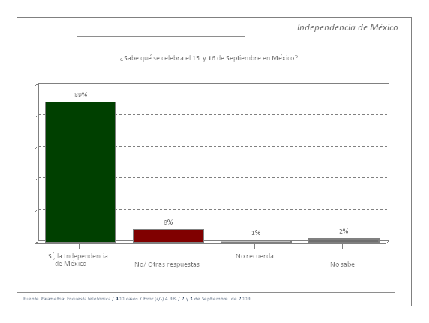
\includegraphics[width=.50\textwidth]{03MarcoTeorico/imageR/enc01}
	\caption{Gráfica a la pregunta ¿Sabe que se celebra el 15 y 16 de Septiembre en México?.}
	\label{fig:enc01}
\end{figure}

\begin{figure}
	\centering 
	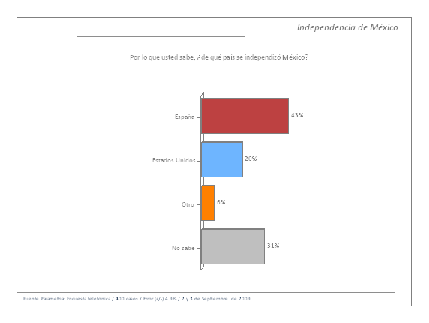
\includegraphics[width=.5\textwidth]{03MarcoTeorico/imageR/enc02}
	\caption{Gráfica a la pregunta ¿De que país se independizó México?.}
	\label{fig:enc02}
\end{figure}

\begin{figure}
	\centering 
	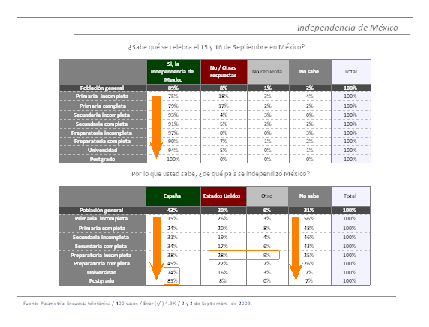
\includegraphics[width=.5\textwidth]{03MarcoTeorico/imageR/enc03}
	\caption{Gráfica de como influye la escolaridad en el conocimiento que se tiene de las fiestas patrias.}
	\label{fig:enc03}
\end{figure}


El movimiento cultural no solo favorecer el desarrollo recreativo si no impulsa el desarrollo de sus naciones.
En otros países del mundo, donde han sabido valorar las costumbres y tradiciones, he ahí donde nace el orgullo por su patria y se convierten en nacionalistas, demostrando el amor por su pueblo, marcando de manera definitiva el desarrollo científico, político, social, de su nación \cite{pp06}.
\\[1pt]

La ignorancia cultural es el principal elemento que permite la injusticia, la enajenación y la explotación. Este fenómeno es sumamente grave y perjudicial para conformar lo que es la Identidad Cultural, la Identidad Nacional y la conciencia de la Nación. Al no saber quién es, cuáles son sus orígenes, su historia, su legado, su nombre, sus valores y principios, se le condena a permanentemente estar exaltando lo ajeno y despreciando lo propio.
\\[1pt]


Tenemos que recuperar nuestro pasado, para poder tener futuro. Debemos saber cuál es nuestra verdadera herencia cultural y cuál nuestro legado, para preservarlo y desarrollarlo. Y como dice Guillermo Marín \cite{pp07} ``Este país se tiene que encontrar a sí mismo. Este país tiene que buscar el espejo humeante de Tezcatlipoca para reconocer su auténtico rostro y su corazón verdadero. Este país tiene que librar una guerra interior para desprender al `Hernán Cortés', que en cada mexicano, se ha ido filtrado en lo profundo de su corazón, y que con un poquito de poder brota violento y resentido contra el hermano más débil o indefenso para vengar las afrentas sufridas durante cinco siglos de dolor e injusticia".
\\[1pt]
